\documentclass[a4paper,12pt]{report}
\usepackage{graphicx}
\usepackage{subfigure}
\usepackage{hyperref}
\usepackage[T1]{fontenc}
\usepackage[utf8]{inputenc}
\usepackage{setspace}
\usepackage[paper=a4paper,margin=1in]{geometry}
\usepackage{float}

\usepackage[backend=biber, sorting=none]{biblatex}

\usepackage{listings}
\usepackage{pacchetti/protobuf/lang}  % include language definition for protobuf
\usepackage{pacchetti/protobuf/style} % include custom style for proto declarations.

\addbibresource{bibliography.bib}
\addbibresource{web.bib}

\begin{document}


    
    \begin{titlepage}
        
        \noindent
        \begin{minipage}[t]{0.19\textwidth}
            \vspace{-4mm}{
\includegraphics[scale=1.15]{images/logo_unimib.pdf}}
        \end{minipage}
        \begin{minipage}[t]{0.81\textwidth}
        {
                \setstretch{1.42}
                {\textsc{Università degli Studi di Milano - Bicocca}} \\
                \textbf{Scuola di Scienze} \\
                \textbf{Dipartimento di Informatica, Sistemistica e Comunicazione} \\
                \textbf{Corso di laurea in Informatica} \\
                \par
        }
        \end{minipage}
        
	\vspace{40mm}
        
	\begin{center}
            {\LARGE{
                    \setstretch{1.2}
                    \textbf{Sistema di controllo  \\ per base robotica outdoor}
                    \par
            }}
        \end{center}
        
        \vspace{50mm}

        \noindent
        {\large \textbf{Relatore:} Prof. Domenico Giorgio Sorrenti } \\

        \noindent
        {\large \textbf{Correlatore:} Dott. Simone Fontana}
        
        \vspace{15mm}

        \begin{flushright}
            {\large \textbf{Relazione della prova finale di:}} \\
            \large{Federica Di Lauro} \\
            \large{Matricola 829470} 
        \end{flushright}
        
        \vspace{40mm}
        \begin{center}
            {\large{\bf Anno Accademico 2019-2020}}
        \end{center}

        \restoregeometry
        
    \end{titlepage}
    

\begin{flushright}
	\textit{ma rompi tutto! \\
            hai rotto l'elettricità \\
            ora è un casino}
\end{flushright}
\newpage

\tableofcontents

\newpage

\chapter{Introduzione}
\chapter{Strumenti}

\section{ROS}

ROS (Robot Operating System) è un framework flessibile usato per scrivere software per robot.
È una collezione di strumenti, librerie e convenzioni che ha lo scopo di semplificare la creazione di sistemi robot complessi e robusti in modo indipendente dalla piattaforma robotica.

ROS è costituito da una rete di processi che vengono eseguiti in parallelo e comunicano tra di loro in modo Peer-to-Peer.
Gli elementi principali che costituiscono il sistema sono:
\begin{itemize}
  \item \textbf{Nodi}: sono i processi che vengono eseguiti in parallelo.
  \item \textbf{Master}: è il server principale che si occupa di effettuare le operazioni di routing per permettere la comunicazione tra i diversi nodi.
  \item \textbf{Messaggi}: il contenuto che si scambiano i nodi. I messaggi possono essere sia di tipo standard sia definiti in modo custom.
  \item \textbf{Topic}: sono il canale di comunicazione usato dai nodi per permettere lo scambio di messaggi.
\end{itemize}
Il sistema di scambio dei messaggi si basa sull'architettura publisher/subscriber: ogni nodo può essere \textit{talker} (Publisher) o \textit{listener}  (Subscriber).
Un nodo talker può creare topic e pubblicare i messaggi su questi canali (sia su topic creati dal nodo steso, sia su topic già esistenti), mentre un nodo listener si sottoscrive ai topic ed esegue una callback ogni volta che viene ricevuto un messaggio. Più nodi listener si possono sottoscrivere allo stesso topic e più nodi talker possono pubblicare sullo stesso topic.

\begin{figure}[H]
\centering
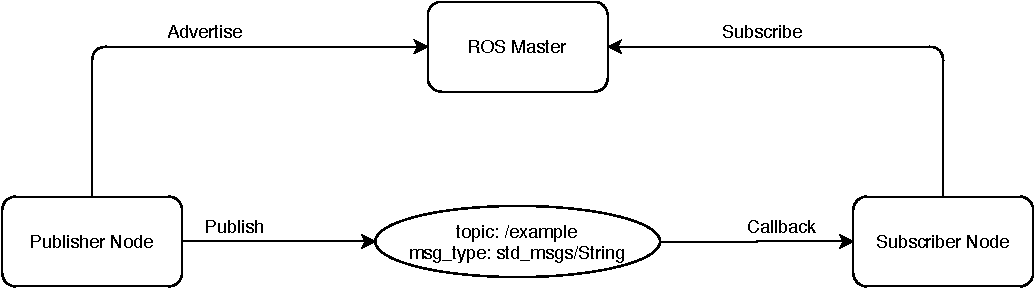
\includegraphics[scale=0.9]{images/ros_system.pdf}
\caption{Schema generale del sistema di comunicazione}
\end{figure}

Il software è open source ed è disponibile sul sito ufficiale \cite{ROS}, la versione usata per questo progetto è la Melodic.

\section{RVIZ}
RVIZ è un tool che permette la visualizzazione 3D dei messaggi scambiati da ROS. Usando questo strumento si può visualizzare in real-time la posizione del robot attraverso i dati dei sensori che vengono pubblicati.

\begin{figure}[H]
\centering
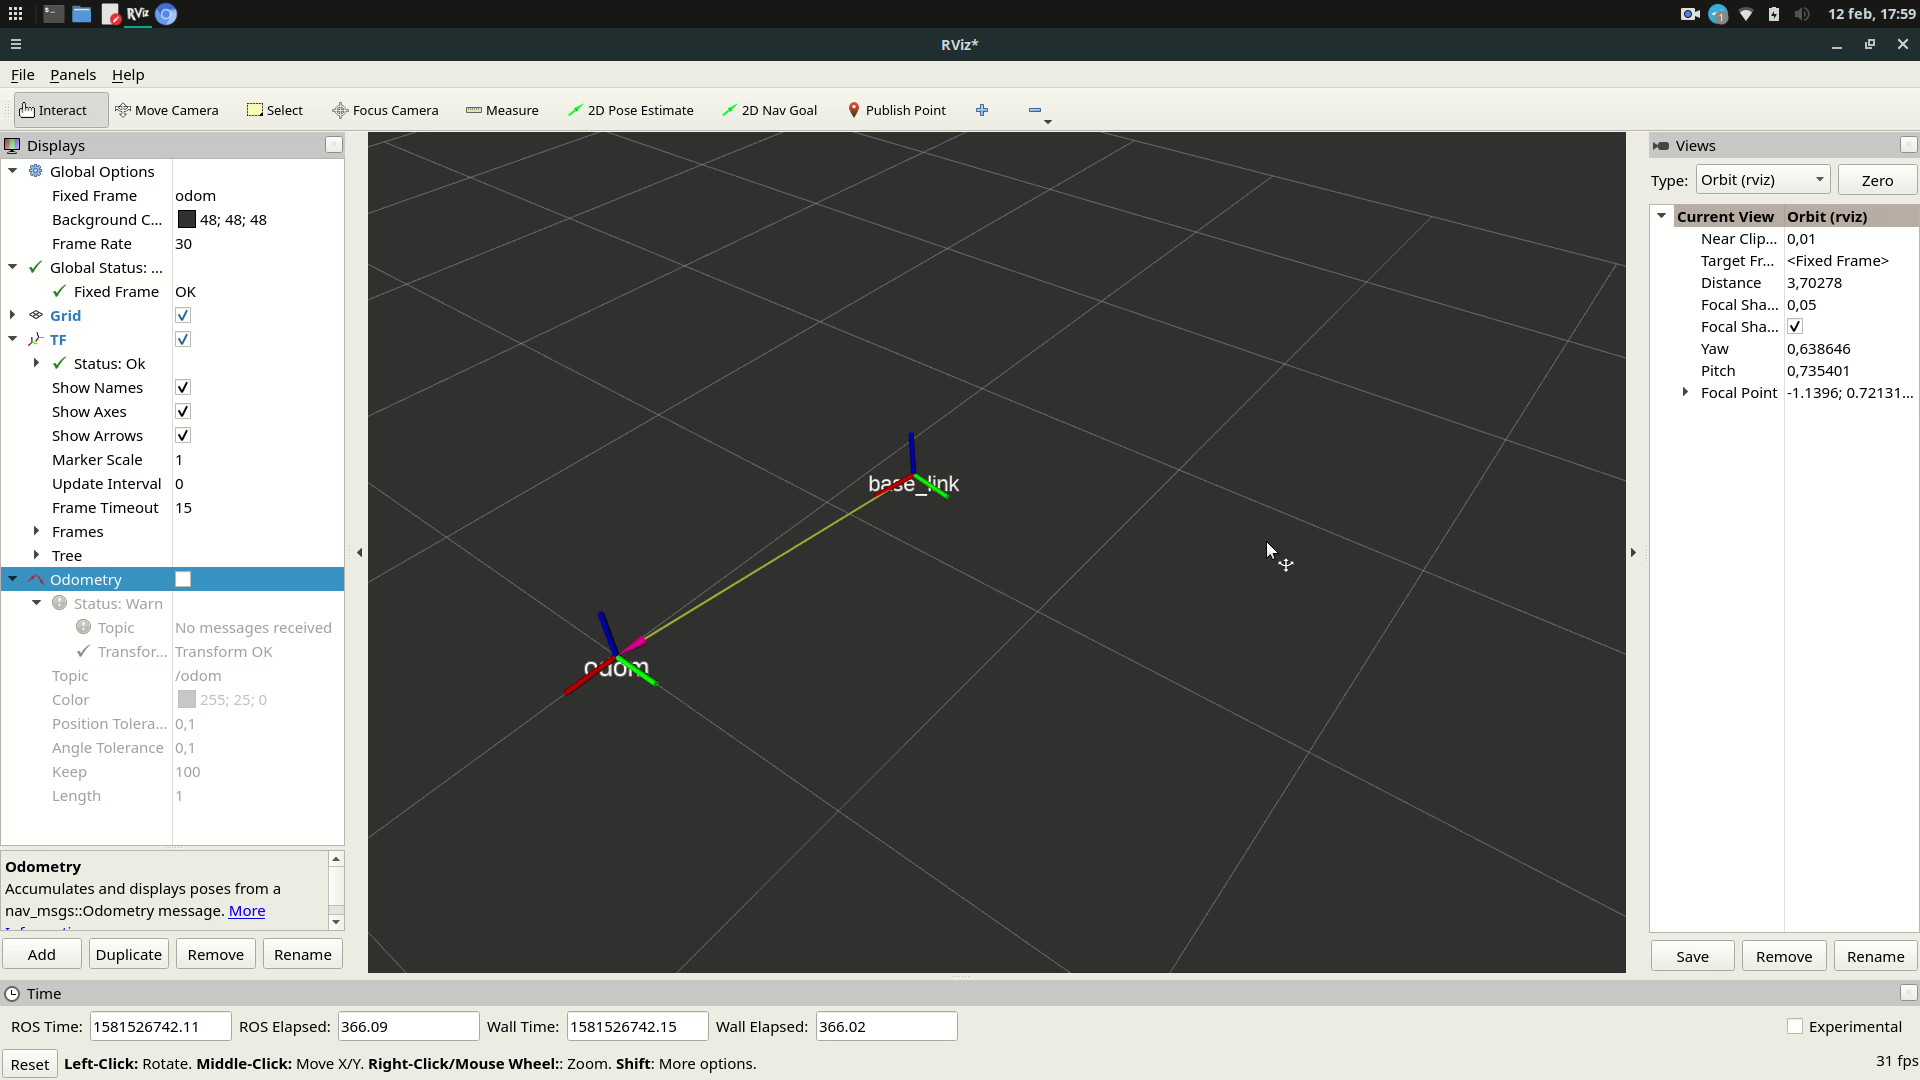
\includegraphics[scale=0.225]{images/rviz.png}
\caption{Visualizzazione di un robot nello spazio con RVIZ}
\end{figure}

\section{STM32CubeIDE}
STM32CubeIDE è un ambiente di sviluppo della ST Microelectronics per la programmazione e il debugging delle schede STM32. Il software è scaricabile gratuitamente dal sito ufficiale \cite{STM32CubeIDE}. \\
Le sue principali caratteristiche sono:
\begin{itemize}
    \item Toolchain GNU C/C++ per Arm e GDB debugger.
    \item Integrazione del tool STM32CubeMX per la generazione del codice di configurazione del sistema e delle periferiche del microcontrollore.
    \item Debugging avanzato che comprende feature come:
    \begin{itemize}
        \item Visualizzazione di CPU core, registri delle periferiche e memoria
        \item Visione delle variabili live 
        \item Analisi del sistema e tracing in tempo reale
        \item Tool di analisi dei CPU fault
    \end{itemize}
\end{itemize}

\begin{figure}[H]
\centering
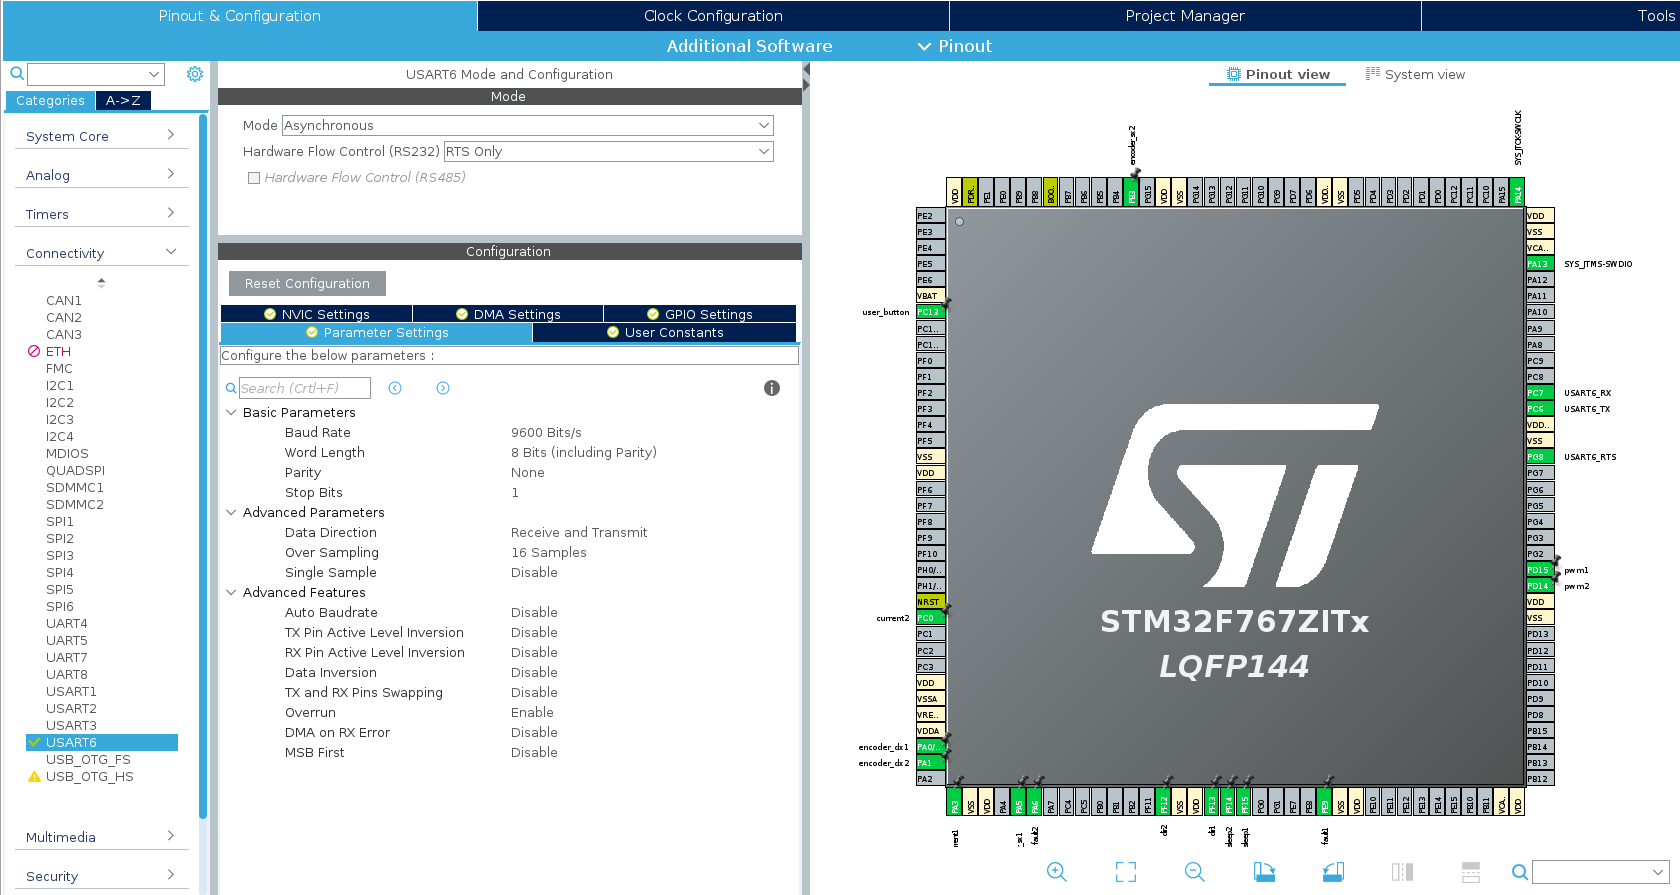
\includegraphics[width=\textwidth]{images/stm32cubemx.png}
\caption{Configurazione di pinout e periferiche tramite lo strumento STM32CubeMX}
\end{figure}

\section{Protocol Buffers}
Protocol Buffers è una libreria per la serializzazione dei dati strutturati, utile per lo sviluppo di software che necessita uno scambio di informazioni tra sistemi indipendenti.
La struttura dei dati viene descritta in un file di tipo \textit{.proto}, dopo di che, attraverso la compilazione con il comando \textit{protoc} e specificando il linguaggio di programmazione desiderato, vengono generate le classi per accedere ai dati. 


\lstinputlisting[language=protobuf2, 
                style=protobuf,
                caption={Esempio di definizione di un messaggio con Protocol Buffers},
                captionpos=b]{codice/esempio.proto}
                
Protocol Buffers è sviluppato da Google e rilasciato con licenza open source \cite{ProtocolBuffers}. \\
Per questo progetto è stata utilizzata anche un'implementazione in C pensata per i microcontrollori, \textit{nanopb} \cite{nanopb}.

\section{sigrok Pulseview}
sigrok è una suite di software per l'analisi dei segnali, sfruttando dispositivi come oscilloscopi e analizzatori logici. 

Pulseview è l'interfaccia grafica usata per sfruttare questi tool e permette di interfacciarsi con i dispositivi sopracitati visualizzando il segnale in tempo reale, analizzandone i tempi e consente inoltre la decodifica di segnali digitali. 

In particolare per questo progetto è stato usato Pulseview con un analizzatore logico per facilitare il debugging nella trasmissione dei segnali, ad esempio la trasmissione seriale di messaggi.

\begin{figure}[H]
\centering
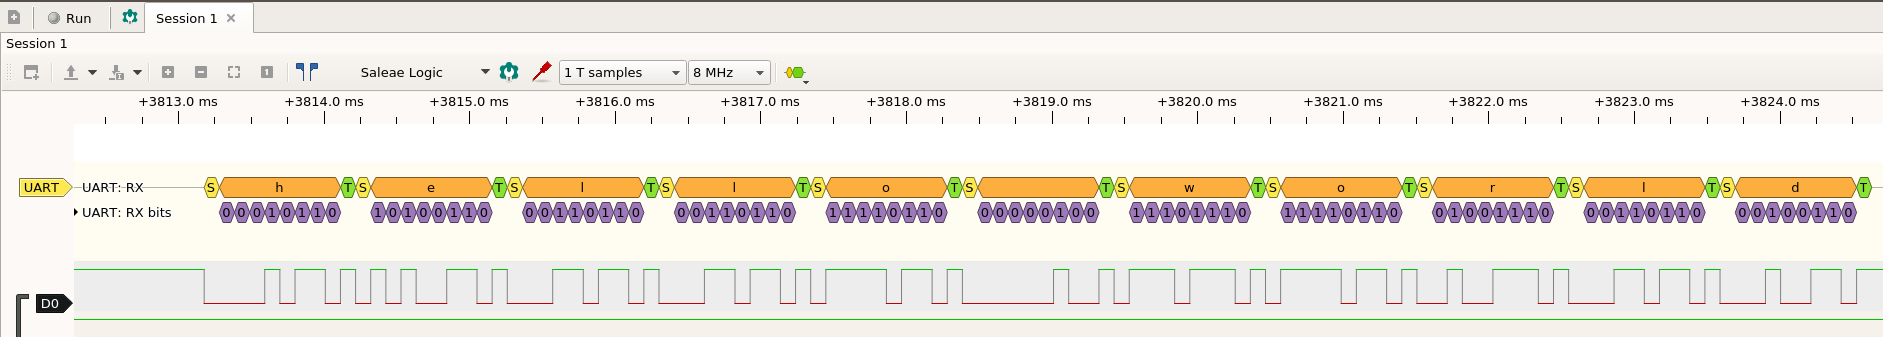
\includegraphics[width=\textwidth]{images/pulseview.png}
\caption{Acquisizione e decodifica di un segnale UART}
\end{figure}

Pulseview è un progetto open source e liberamente scaricabile dal sito ufficiale\cite{Pulseview}.
\chapter{Base robotica Otto}

Otto è un robot a guida differenziale, progetto di ricerca del laboratorio di robotica IRALab, dell’Università degli Studi di Milano-Bicocca.

\section{Base robotica VolksBot RT 3}
VolksBot è un kit modulare per la costruzione di robot, progettato per il campo della ricerca e della  prototipazione rapida.
La base robotica è pensata per essere facilmente modificata ed adattata alle proprie esigenze in quanto composta da barre in alluminio combinabili fra di loro.

Nello specifico la base robotica utilizzata è composta da due ruote motrici frontali e una ruota basculante di supporto posteriore.
Ciascuna ruota motrice è collegata ad un motore a corrente continua combinato con una riduzione con un rapporto di trasmissione 1:74.
L'intero sistema robotico è alimentato tramite batterie a bordo del veicolo.
\begin{figure}[H]
\centering
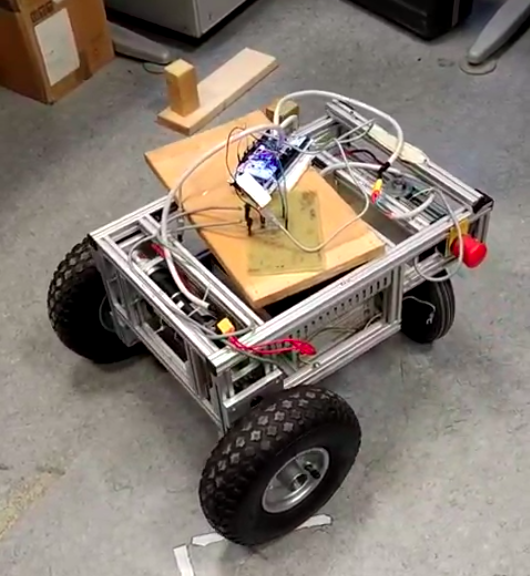
\includegraphics[scale=0.45]{images/otto1.png}
\caption{Base robotica Otto}
\end{figure}

\section{Encoder}
Un encoder è dispositivo elettromeccanico in grado di convertire la posizione o il moto angolare in un codice digitale.

Nel nostro caso è stato montato un encoder in quadratura sull'asse del motore di ciascuna ruota motrice.
Questo tipo di sensore è formato da un LED, da una corona circolare con un pattern fisso che si ripete e da dei fotodiodi. 

\begin{figure}[H]
\centering
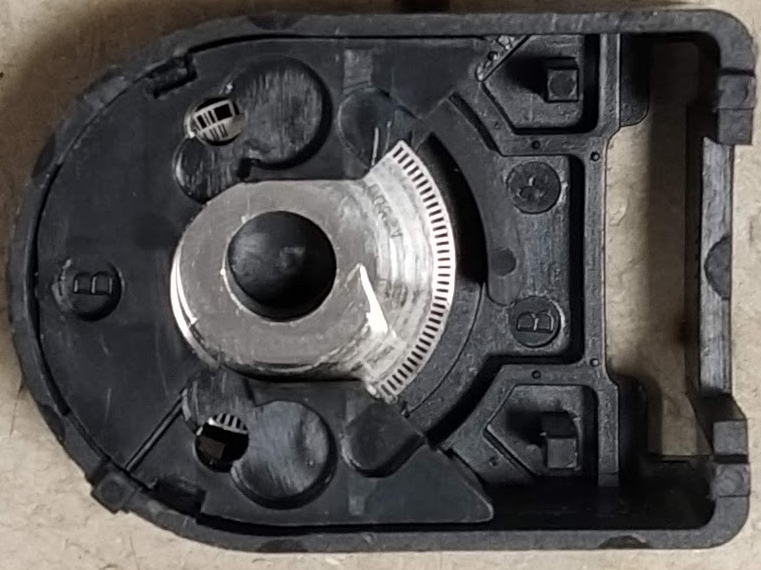
\includegraphics[scale=0.30]{images/corona.png}
\caption{Corona circolare dell'encoder}
\end{figure}

Il funzionamento si basa sulla capacità dei fotodiodi di percepire i cambiamenti di luce: il LED viene sempre alimentato ed emette quindi una luce costante, la corona dell'encoder gira insieme all'albero del motore e i fotodiodi rilevano i cambiamenti di luce dovuti al pattern sulla corona e tramite dei comparatori generano delle onde quadre.
Elaborando questi segnali è possibile misurare sia la distanza percorsa dalle ruote che la direzione del movimento.

\begin{figure}[H]
\hfill
\subfigure[Schema dell'encoder]{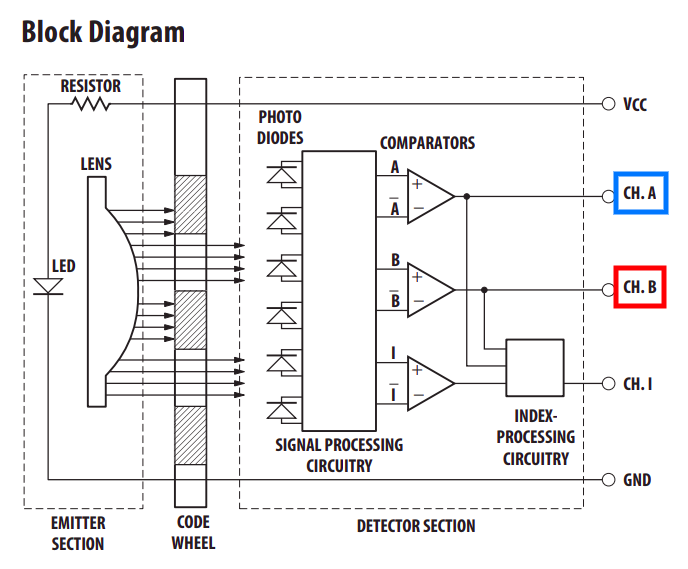
\includegraphics[scale=0.32]{images/encoder-1.png}}
\hfill
\subfigure[Segnale generato]{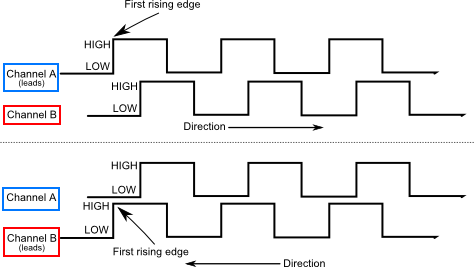
\includegraphics[scale=0.47]{images/quad-encoding-waveform-1.png}}
\hfill
\caption{Encoder in quadratura}
\end{figure}

\section{Motor driver}
Un motor driver è un dispositivo elettronico necessario per poter controllare i motori DC usando i segnali digitali generati da un microcontrollore.
Il circuito elettronico principale è chiamato ponte H e permette di controllare la polarità della tensione applicata a un carico. Tramite questo meccanismo siamo in grado sia di controllare la direzione del moto di un motore a corrente continua, stabilendo il verso nel quale fluisce la corrente, sia di regolare la velocità del motore modulando la tensione.

La modulazione della tensione avviene tramite un segnale PWM (pulse-width modulation). Questo segnale periodico ha due fasi: una in cui la tensione è alta (3.3V) e una fase in cui la tensione è bassa (0V). Il rapporto tra queste due fasi è detto duty-cycle e determina la tensione media in uscita.

\begin{figure}[H]
\centering
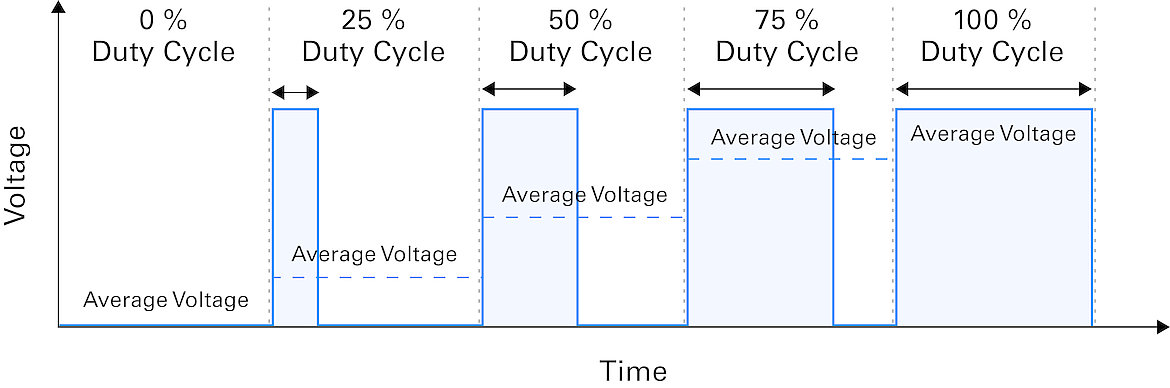
\includegraphics[width=\textwidth]{images/pwm.jpg}
\caption{Modulazione della tensione con segnale PWM.}
\end{figure}


Il motor driver scelto è Pololu Dual G2: questo dispositivo ha due circuiti H-bridge, così da poter controllare entrambi i motori in modo indipendente.
Per controllare ciascun motore sono presenti 3 segnali di input:
\begin{itemize}
    \item SLP: disabilita l'output se è uguale a 0
    \item PWM: input particolare rappresentabile come percentuale, modula la velocità
    \item DIR: imposta la direzione di azione del motore
\end{itemize}

Si hanno quindi le seguenti modalità di funzionamento:
\begin{table}[H]
    \centering
    \begin{tabular}{|l|l|l|l|}
    \hline
    SLP & DIR & PWM & Operazione                            \\ \hline
    1   & 0   & \%pwm & motore azionato in senso orario a velocità pwm \\
    1   & 1   & \%pwm & motore azionato in senso antiorario a velocità pwm         \\
    1   & x   & 0   & motore frenato                        \\
    0   & x   & x   & motore libero                     \\ \hline
    \end{tabular}
\end{table}

Sono inoltre presenti due segnali analogici di output per controllare il consumo dei motori (CS) e due segnali di output per monitorare lo stato di eventuali guasti (FLT).

\begin{figure}[H]
\centering
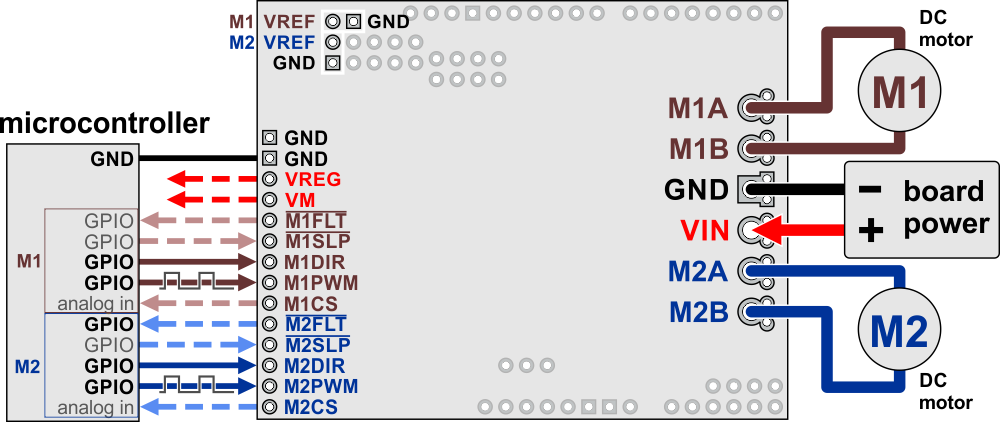
\includegraphics[scale=1.4]{images/pololu.png}
\caption{Schema delle connessioni del Pololu Dual G2.}
\end{figure}


\section{Microcontrollore}
La scheda di sviluppo scelta è una Nucleo STM32F767ZI.
Il processore è un Core Arm 32-bit Cortex-M7, ed è presente una Floating Point Unit per velocizzare le operazioni in virgola mobile.
La scheda ha 512kB di memoria RAM e 2MB di memoria FLASH.
È stata scelta per la grande disponibilità di periferiche integrate, in particolare per la realizzazione del sistema di controllo sono stati necessari: 
\begin{itemize}
    \item 2 timer a 32 bit per la gestione degli encoder.
    \item 1 timer a 16 bit per la generazione del segnale PWM.
    \item 1 periferica UART per la comunicazione con il computer.
\end{itemize}
Inoltre è presente un debugger integrato ST-LINK V2.1.

\begin{figure}[H]
\centering
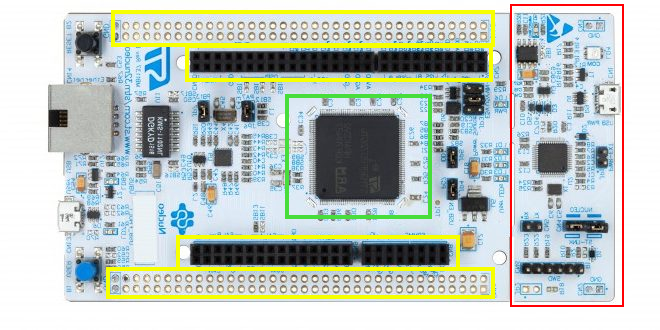
\includegraphics[scale=0.65]{images/nucleo.png}
\caption{La scheda Nucleo. Evidenziato in rosso il debugger, in verde il processore ed in giallo i GPIO per interfacciarsi con le varie periferiche.}
\end{figure}

\section{Modulo FTDI}
Per quanto riguarda la comunicazione tra microcontrollore e computer si è scelto il protocollo UART. 
Per rendere il sistema utilizzabile collegando un qualsiasi computer è stato necessario un modulo apposito che convertisse il segnale UART in un segnale USB, così da non dover utilizzare una piattaforma apposita dotata di GPIO.

È stato utilizzato un modulo FTDI FT232RL in quanto ampiamente supportato a livello di driver Linux e perché, oltre alle linee di trasmissione e ricezione, presenta alcuni meccanismi di controllo del flusso hardware tramite appositi pin (CTS e RTS) e un pin per poter effettuare il reset del microcontrollore direttamente dal PC.


\begin{figure}[H]
\centering
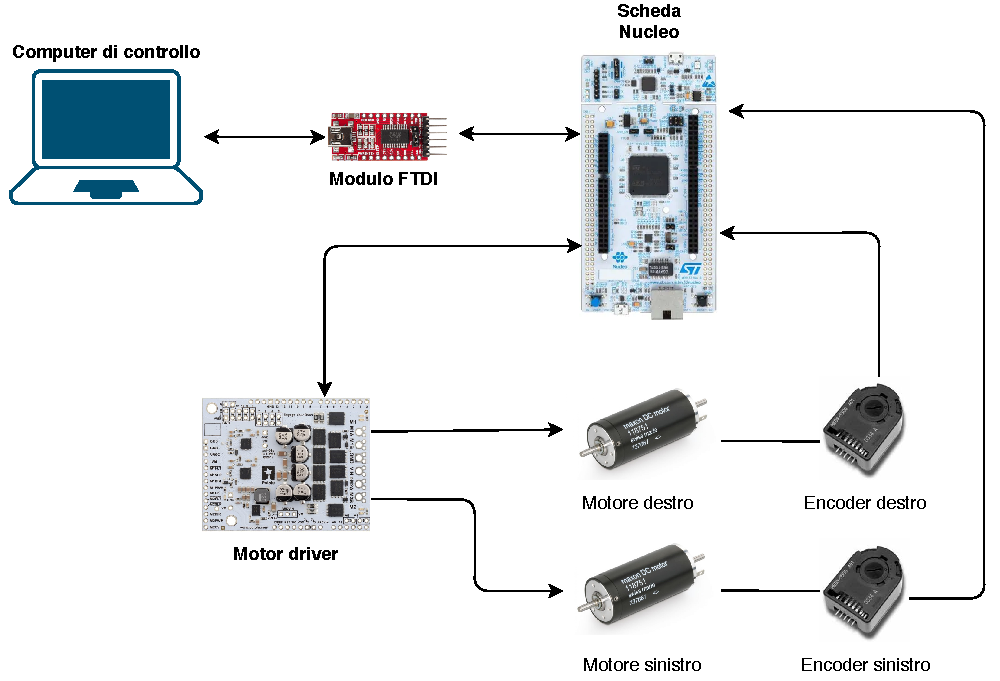
\includegraphics[width=\textwidth]{images/infrastruttura.pdf}
\caption{Riepilogo generale dei componenti e delle loro connessioni.}
\end{figure}

\chapter{Sviluppo}

\section{Progettazione del sistema}
L'obiettivo di questo stage è stato la creazione del sistema di controllo di un robot a guida differenziale che si integrasse con il framework ROS.
Innanzitutto è stata necessaria un'analisi dei requisiti, nella quale sono stati individuati i seguenti punti: 
\begin{itemize}
    \item Elaborazione dei dati degli encoder per ricavare l'odometria del robot.
    \item Controllo dei motori tramite un sistema di retroazione.
    \item Comunicazione bidirezionale con un computer di controllo.
\end{itemize}

Per l'ultimo punto è stato necessario studiare un sistema per poter integrare la comunicazione con il framework ROS, in particolare per poter utilizzare il Navigation Stack.
Lo stack di navigazione è molto semplice a livello concettuale. Esso riceve le informazioni riguardanti l'odometria e i dati dei sensori, e restituisce in output i comandi che il robot deve eseguire.

\begin{figure}[h]
    \centering
    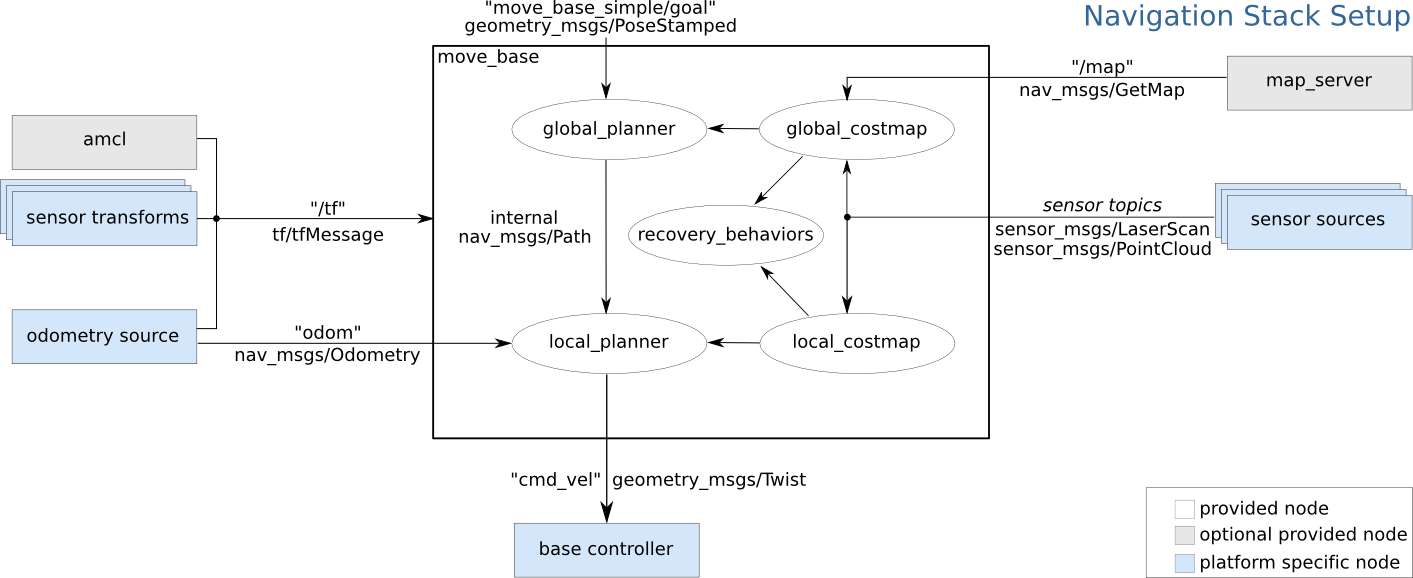
\includegraphics[scale=0.38]{images/navigation_stack.png}
    \caption{Lo schema dello stack di navigazione. Come mostrato nella legenda, i nodi in
bianco sono quelli già forniti, quelli in grigio sono opzionali e quelli in blu sono specifici per il singolo robot che devono essere implementati.}
  \label{fig:navigation_stack}
\end{figure}

\newpage
Come illustrato nella figura \ref{fig:navigation_stack} i messaggi da pubblicare, per quanto riguarda il sistema di controllo, sono messaggi di tipo \textit{nav\_msgs/Odometry} sul topic \textit{/odom} e i messaggi di tipo \textit{tf/Message} sul topic \textit{/tf}, e bisogna sottoscriversi ai messaggi di tipo \textit{geometry\_msgs/Twist} sul topic \textit{/cmd\_vel}. \\
Il messaggio \textit{Odometry} contiene le informazioni riguardanti la pose del robot nello spazio, prendendo come sistema di riferimento la prima posizione del robot ed è composto da:
\begin{itemize}
    \item Posizione espressa come \textit{x, y, z}
    \item Orientamento espresso come \textit{quaternion}
    \item Velocità lineare e velocità angolare attuali
\end{itemize}
Il messaggio \textit{tf} contiene le informazioni riguardanti pose del robot ed è necessario in quanto ci permette di rappresentare l'albero delle trasformazioni delle varie parti del robot, ovvero le posizioni relative delle varie parti come laser e altri sensori rispetto alla base mobile, chiamata \textit{base\_link} \\
Il messaggio \textit{geometry\_msgs/Twist} contiene le informazioni per far muovere il robot, nel caso di un robot a guida differenziale queste informazioni sono la velocità lineare sull'asse delle x, e la velocità angolare rispetto all'asse delle z.

Si è scelto di far gestire la parte relativa allo scambio dei messaggi ROS al computer principale, che comunica con la scheda di controllo tramite il modulo usb-seriale. 
Sono stati creati due nodi ROS, uno che si sottoscrive al topic \textit{/cmd\_vel} e trasmette i comandi alla scheda, e un nodo che riceve le informazioni relative alla velocità del robot, le elabora e pubblica i messaggi su \textit{/odom} e \textit{/tf}. \\
Il microcontrollore deve svolgere tre compiti: 
\begin{itemize}
    \item Gestire i loop di controllo PID per la gestione dei motori.
    \item Ricevere i comandi, ricavare i valori delle velocità dei motori e impostare quindi i setpoint dei controlli PID.
    \item Inviare i dati di odometria.
\end{itemize}

La trasmissione dei dati di odometria avviene periodicamente leggendo i dati degli encoder, mentre l'aggiornamento dei comandi da far eseguire ai motori avviene in modo asincrono ogni volta che il messaggio di comando viene ricevuto.

\section{Implementazione microcontrollore}
\subsection{Struttura del codice}
Lo scheletro del codice e l'inizializzazione delle periferiche sono stati generati tramite allo strumento STM32CubeMX. Il software è stato scritto in C++ per permettere un miglior riutilizzo del codice attraverso l'utilizzo delle classi.

\begin{figure}[H]
    \centering
    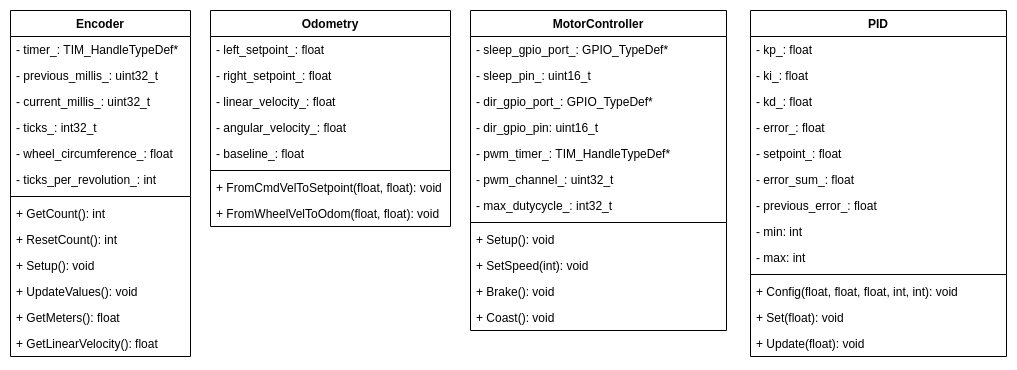
\includegraphics[scale=0.44]{images/diagramma_classi.png}
    \caption{Diagramma delle classi}
\end{figure}


\subsection{Lettura encoder}
\subsection{Controllo PID dei motori}
\cite{cross_pid}
\subsection{Comunicazione seriale con computer}
\section{Implementazione nodi ROS}
\section{Testing}

\chapter{Conclusioni}

\newpage
\printbibheading[heading=bibintoc, title={Riferimenti}]
\printbibliography[nottype=online,heading=subbibintoc,title={Bibliografia}]
\printbibliography[type=online,heading=subbibintoc,title={Siti}]

\appendix
\chapter{Lista delle parti}

\textbf{Base robotica:}
\begin{itemize}
    \item Base robotica Volksbot RT 3
    \item Dimensioni: 580 x 520 x 315 mm
    \item Dimensione baseline: 435 mm
    \item Peso (escluse batterie): 17kg
    \item Ruote 260 x 85 mm, ruota di supporto piroettante 200mm
    \item Circonferenza ruote misurato a 3 bar: 783mm
    \item Batterie al piombo 12V, 15AH
\end{itemize}
\textbf{Motori:}
\begin{itemize}
    \item Motori Maxon RE 40 Ø40 mm, Graphite Brushes, 150 Watt
    \item Riduzioni 1:74 Planetary Gearhead GP 42 C Ø42 mm, 3 - 15 Nm, Ceramic Version
    \item Encoder HEDS-5540\#A11
\end{itemize}
\textbf{Elettronica:}
\begin{itemize}
    \item Scheda di controllo Nucleo F767ZI
    \item Modulo seriale FTDI FT232RL
    \item Motor driver Pololu Dual G2 High-Power Motor Driver 24v18 Shield
    \item PCB custom disegnata con KiCad, disponibile sulla repo del progetto
\end{itemize}

\end{document}
